% Created by tikzDevice version 0.7.0 on 2015-04-28 10:39:23
% !TEX encoding = UTF-8 Unicode
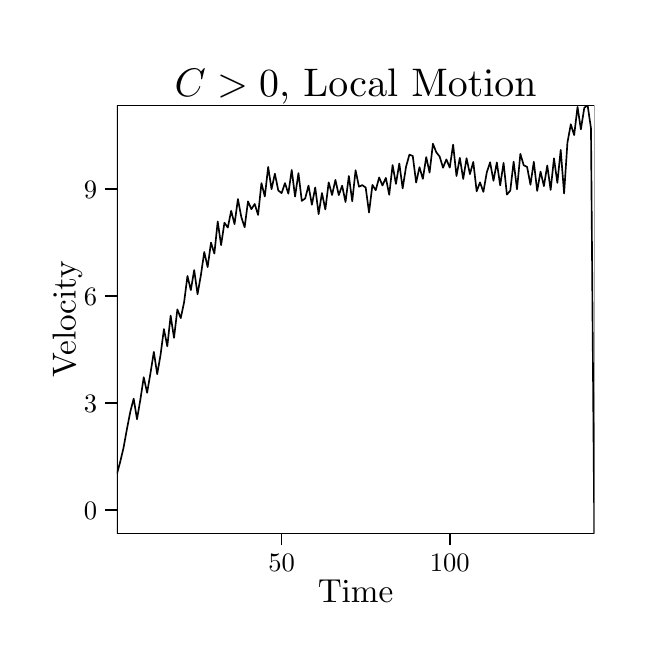
\begin{tikzpicture}[x=1pt,y=1pt]
\definecolor[named]{fillColor}{rgb}{1.00,1.00,1.00}
\path[use as bounding box,fill=fillColor,fill opacity=0.00] (0,0) rectangle (216.81,216.81);
\begin{scope}
\path[clip] (  0.00,  0.00) rectangle (216.81,216.81);
\definecolor[named]{drawColor}{rgb}{1.00,1.00,1.00}
\definecolor[named]{fillColor}{rgb}{1.00,1.00,1.00}

\path[draw=drawColor,line width= 0.6pt,line join=round,line cap=round,fill=fillColor] ( -0.00,  0.00) rectangle (216.81,216.81);
\end{scope}
\begin{scope}
\path[clip] ( 32.22, 34.03) rectangle (204.76,188.82);
\definecolor[named]{fillColor}{rgb}{1.00,1.00,1.00}

\path[fill=fillColor] ( 32.22, 34.03) rectangle (204.76,188.82);
\definecolor[named]{drawColor}{rgb}{0.00,0.00,0.00}

\path[draw=drawColor,line width= 0.6pt,line join=round] ( 32.22, 55.39) --
	( 33.44, 59.94) --
	( 34.65, 65.06) --
	( 35.87, 71.79) --
	( 37.08, 78.01) --
	( 38.30, 82.76) --
	( 39.51, 75.34) --
	( 40.73, 82.47) --
	( 41.94, 90.48) --
	( 43.16, 84.89) --
	( 44.37, 91.96) --
	( 45.59, 99.67) --
	( 46.80, 91.61) --
	( 48.02, 98.59) --
	( 49.23,107.90) --
	( 50.45,101.67) --
	( 51.66,112.73) --
	( 52.88,104.72) --
	( 54.09,115.01) --
	( 55.31,111.86) --
	( 56.52,117.58) --
	( 57.74,127.08) --
	( 58.95,121.99) --
	( 60.17,129.21) --
	( 61.38,120.48) --
	( 62.60,127.45) --
	( 63.81,135.75) --
	( 65.03,130.29) --
	( 66.24,139.12) --
	( 67.46,135.19) --
	( 68.67,146.76) --
	( 69.89,138.25) --
	( 71.10,146.33) --
	( 72.32,144.56) --
	( 73.53,150.63) --
	( 74.75,145.83) --
	( 75.97,154.88) --
	( 77.18,148.43) --
	( 78.40,144.70) --
	( 79.61,154.04) --
	( 80.83,151.23) --
	( 82.04,153.10) --
	( 83.26,149.14) --
	( 84.47,160.62) --
	( 85.69,155.80) --
	( 86.90,166.47) --
	( 88.12,158.46) --
	( 89.33,164.03) --
	( 90.55,157.98) --
	( 91.76,157.04) --
	( 92.98,160.65) --
	( 94.19,156.82) --
	( 95.41,165.39) --
	( 96.62,155.78) --
	( 97.84,164.25) --
	( 99.05,154.23) --
	(100.27,155.09) --
	(101.48,159.73) --
	(102.70,152.83) --
	(103.91,159.07) --
	(105.13,149.46) --
	(106.34,157.04) --
	(107.56,151.13) --
	(108.77,160.91) --
	(109.99,156.34) --
	(111.20,161.80) --
	(112.42,156.30) --
	(113.63,159.72) --
	(114.85,153.82) --
	(116.06,163.21) --
	(117.28,154.11) --
	(118.49,165.29) --
	(119.71,159.33) --
	(120.92,159.91) --
	(122.14,159.03) --
	(123.35,150.02) --
	(124.57,159.98) --
	(125.78,158.07) --
	(127.00,162.68) --
	(128.21,159.79) --
	(129.43,162.52) --
	(130.64,156.42) --
	(131.86,167.16) --
	(133.07,160.36) --
	(134.29,167.72) --
	(135.50,158.76) --
	(136.72,166.53) --
	(137.93,170.91) --
	(139.15,170.45) --
	(140.37,160.85) --
	(141.58,166.39) --
	(142.80,162.17) --
	(144.01,170.04) --
	(145.23,164.46) --
	(146.44,174.87) --
	(147.66,171.76) --
	(148.87,170.24) --
	(150.09,166.20) --
	(151.30,169.22) --
	(152.52,166.25) --
	(153.73,174.56) --
	(154.95,163.21) --
	(156.16,169.78) --
	(157.38,162.15) --
	(158.59,169.61) --
	(159.81,163.90) --
	(161.02,168.29) --
	(162.24,157.67) --
	(163.45,160.92) --
	(164.67,157.46) --
	(165.88,164.41) --
	(167.10,168.17) --
	(168.31,161.51) --
	(169.53,168.10) --
	(170.74,159.81) --
	(171.96,167.95) --
	(173.17,156.48) --
	(174.39,157.93) --
	(175.60,168.38) --
	(176.82,158.43) --
	(178.03,171.19) --
	(179.25,167.07) --
	(180.46,166.49) --
	(181.68,160.07) --
	(182.89,168.35) --
	(184.11,157.82) --
	(185.32,164.80) --
	(186.54,159.57) --
	(187.75,167.02) --
	(188.97,158.17) --
	(190.18,169.59) --
	(191.40,160.74) --
	(192.61,172.64) --
	(193.83,156.91) --
	(195.04,175.29) --
	(196.26,181.89) --
	(197.47,177.98) --
	(198.69,188.18) --
	(199.90,180.06) --
	(201.12,187.80) --
	(202.33,188.82) --
	(203.55,180.40) --
	(204.76, 34.03);

\path[draw=drawColor,line width= 0.6pt,line join=round,line cap=round] ( 32.22, 34.03) rectangle (204.76,188.82);
\end{scope}
\begin{scope}
\path[clip] (  0.00,  0.00) rectangle (216.81,216.81);
\definecolor[named]{drawColor}{rgb}{0.00,0.00,0.00}

\node[text=drawColor,anchor=base east,inner sep=0pt, outer sep=0pt, scale=  0.96] at ( 25.11, 39.15) {0};

\node[text=drawColor,anchor=base east,inner sep=0pt, outer sep=0pt, scale=  0.96] at ( 25.11, 77.81) {3};

\node[text=drawColor,anchor=base east,inner sep=0pt, outer sep=0pt, scale=  0.96] at ( 25.11,116.47) {6};

\node[text=drawColor,anchor=base east,inner sep=0pt, outer sep=0pt, scale=  0.96] at ( 25.11,155.12) {9};
\end{scope}
\begin{scope}
\path[clip] (  0.00,  0.00) rectangle (216.81,216.81);
\definecolor[named]{drawColor}{rgb}{0.00,0.00,0.00}

\path[draw=drawColor,line width= 0.6pt,line join=round] ( 27.95, 42.46) --
	( 32.22, 42.46);

\path[draw=drawColor,line width= 0.6pt,line join=round] ( 27.95, 81.12) --
	( 32.22, 81.12);

\path[draw=drawColor,line width= 0.6pt,line join=round] ( 27.95,119.77) --
	( 32.22,119.77);

\path[draw=drawColor,line width= 0.6pt,line join=round] ( 27.95,158.43) --
	( 32.22,158.43);
\end{scope}
\begin{scope}
\path[clip] (  0.00,  0.00) rectangle (216.81,216.81);
\definecolor[named]{drawColor}{rgb}{0.00,0.00,0.00}

\path[draw=drawColor,line width= 0.6pt,line join=round] ( 91.76, 29.77) --
	( 91.76, 34.03);

\path[draw=drawColor,line width= 0.6pt,line join=round] (152.52, 29.77) --
	(152.52, 34.03);
\end{scope}
\begin{scope}
\path[clip] (  0.00,  0.00) rectangle (216.81,216.81);
\definecolor[named]{drawColor}{rgb}{0.00,0.00,0.00}

\node[text=drawColor,anchor=base,inner sep=0pt, outer sep=0pt, scale=  0.96] at ( 91.76, 20.31) {50};

\node[text=drawColor,anchor=base,inner sep=0pt, outer sep=0pt, scale=  0.96] at (152.52, 20.31) {100};
\end{scope}
\begin{scope}
\path[clip] (  0.00,  0.00) rectangle (216.81,216.81);
\definecolor[named]{drawColor}{rgb}{0.00,0.00,0.00}

\node[text=drawColor,anchor=base,inner sep=0pt, outer sep=0pt, scale=  1.20] at (118.49,  9.03) {Time};
\end{scope}
\begin{scope}
\path[clip] (  0.00,  0.00) rectangle (216.81,216.81);
\definecolor[named]{drawColor}{rgb}{0.00,0.00,0.00}

\node[text=drawColor,rotate= 90.00,anchor=base,inner sep=0pt, outer sep=0pt, scale=  1.20] at ( 17.30,111.43) {Velocity};
\end{scope}
\begin{scope}
\path[clip] (  0.00,  0.00) rectangle (216.81,216.81);
\definecolor[named]{drawColor}{rgb}{0.00,0.00,0.00}

\node[text=drawColor,anchor=base,inner sep=0pt, outer sep=0pt, scale=  1.44] at (118.49,191.84) {$C > 0$, Local Motion};
\end{scope}
\end{tikzpicture}
